\documentclass{article}
\usepackage[utf8]{inputenc}
\usepackage[T1]{fontenc}
\usepackage[brazil]{babel}
\usepackage{geometry}
\usepackage{graphicx}
\usepackage{float}
\usepackage{array}
\usepackage{booktabs}
\usepackage{amsmath}
\usepackage{hyperref}

\title{Roteiro 1}
\author{Ana Beatriz Barbosa Yoshida - RA: 245609 \\ Julio Nunes Avelar - RA: 241163}
\date{Agosto de 2025}

\begin{document}

\maketitle

\tableofcontents
\newpage

% ---------------- Experiência 1 ----------------
\section{Experiência 1}

\subsection{1.1 Identificação das GPIOs do LED RGB}
\textbf{Pergunta:} Identifique as GPIOs que estão conectadas no LED RGB da BitDogLab. \\


\textbf{Resposta:} As conexões do LED RGB com resistores de proteção estão descritas a seguir:  
\begin{itemize}
    \item Vermelho: GPIO 13 com resistor de 220 $\Omega$
    \item Verde: GPIO 11 com resistor de 220 $\Omega$
    \item Azul: GPIO 12 com resistor de 150 $\Omega$
\end{itemize}

\subsection{1.2 Níveis lógicos do RP2040}
\textbf{Pergunta:} Qual a tensão de saída de cada nível lógico do RP2040? \\

\textbf{Resposta:} Os níveis lógicos do microcontrolador RP2040 são:  
\begin{itemize}
    \item Nível lógico 0: 0 V
    \item Nível lógico 1: 3.3 V
\end{itemize}

\subsection{1.3 Circuito básico e cálculo dos resistores}
\textbf{Pergunta:} Desenhe o circuito básico para acender este LED com as GPIOs. Calcule o valor de cada resistor. \\

\textbf{Resposta:} O circuito básico do LED RGB está ilustrado na Figura \ref{fig:circuito_led}.  

\begin{figure}[H]
    \centering
    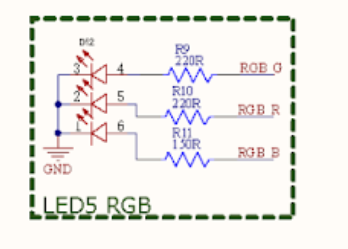
\includegraphics[width=0.6\textwidth]{circuito_led.png}
    \caption{Circuito do LED RGB com resistores.}
    \label{fig:circuito_led}
\end{figure}

O cálculo dos resistores é feito pela Lei de Ohm:  
\[
R = \frac{V_{CC} - V_{LED}}{I_{LED}}
\]

Os valores de corrente e tensão utilizados para cada cor do Led RGB podem ser encontrados no datasheet do Led

\subsection{Tarefa 1.1 -- Comparação entre linguagens}
\textbf{Pergunta:} Comparar o tempo de resposta e fluxo de execução entre C e MicroPython. Sugira um método para obter esses valores e crie uma tabela para realizarmos um Benchmark. \\

\textbf{Resposta:}  
Para realizar o Benchmark entre as duas implementações (C e MicroPython), podemos analisar o tempo gasto para executar rotinas simples, como configuração de GPIOs, execução de funções básicas (acender um LED, imprimir uma string) e cálculos matemáticos. Os resultados obtidos estão apresentados na Tabela \ref{tab:benchmark}.  

\begin{table}[H]
    \centering
    \label{tab:benchmark}
    \begin{tabular}{lcc}
        \toprule
        Linguagem & Tempo ($\mu$s) & Teste \\
        \midrule
        C            & 13       & Inicialização das GPIOs \\
        MicroPython  & 452      & Inicialização das GPIOs \\
        C            & 10010890 & Loop com blink (10 iterações) \\
        MicroPython  & 10000689 & Loop com blink (10 iterações) \\
        C            & 246757   & Verificação de primos \\
        MicroPython  & 1226509  & Verificação de primos \\
        \bottomrule
    \end{tabular}
    \caption{Benchmark básico entre C e MicroPython.}
\end{table}

\subsection{Tarefa 1.2 -- Comparativo Imperativo vs OO}
\textbf{Pergunta:} Comparar tamanho do código (em bytes), tempo de resposta e fluxo de execução entre os modos imperativo e OO para ambos: MicroPython e C. Sugira um método para obter esses valores e crie uma tabela para realizarmos um Benchmark.  \\

\textbf{Resposta:}  
Uma comparação direta do tamanho do código em bytes não é apropriada, pois se trata de linguagens e paradigmas diferentes. Técnicas de escrita distintas podem resultar em códigos mais ou menos verbosos. No caso do C, a implementação de OO (via ponteiros de funções, structs com métodos ou C++) é amplamente otimizada pelo compilador, reduzindo overhead em tempo de execução.  

Ainda assim, é possível avaliar a diferença de desempenho comparando implementações imperativas e orientadas a objetos quanto ao tempo de resposta e eficiência. Essa análise está resumida na Tabela \ref{tab:benchmark_oo}.  

\begin{table}[H]
    \centering
    \label{tab:benchmark_oo}
    \begin{tabular}{lcccc}
        \toprule
        Paradigma & Linguagem & Tamanho Código (bytes) & Tempo de Resposta ($\mu$s) & Observações \\
        \midrule
        Imperativo & C        & ... & ... & ... \\
        OO         & C        & ... & ... & ... \\
        Imperativo & Python   & ... & ... & ... \\
        OO         & Python   & ... & ... & ... \\
        \bottomrule
    \end{tabular}
    \caption{Benchmark entre Imperativo e OO em C e Python.}
\end{table}

% ---------------- Experiência 2 ----------------
\section{Experiência 2}

\subsection{2.1 GPIOs conectados aos botões}
\textbf{Pergunta:} Identifique as GPIOs que estão conectadas aos 3 botões.  

\textbf{Resposta:}  
A identificação está apresentada na Tabela \ref{tab:botoes}.  

\begin{table}[H]
    \centering
    \begin{tabular}{ccc}
        \toprule
         Botão & IO   & Função \\
         \midrule
         RESET  & RUN  & Reset do Pi Pico \\
         Botão A & GP05 & Botão genérico \\
         Botão B & GP06 & Botão genérico \\
         Botão C & GP10 & Botão genérico \\
        \bottomrule
    \end{tabular}
    \caption{Mapeamento dos botões conectados ao RP2040.}
    \label{tab:botoes}
\end{table}

\subsection{2.2 Limites de tensão para nível lógico}
\textbf{Pergunta:} Quais os limites de tensão considerados como nível baixo e alto no microcontrolador utilizado? \\ 

\textbf{Resposta:}  
\begin{itemize}
    \item Nível baixo: $V < V_{IL(max)}$
    \item Nível alto: $V > V_{IH(min)}$
\end{itemize}

Com $V_{IL(max)}$ sendo 0.8V e $V_{IH(min)}$ sendo 2.0V.

\subsection{2.3 Esquema dos botões}
\textbf{Pergunta:} Represente como os botões estão conectados ao microcontrolador.  \\

\textbf{Resposta:}  
O esquema está mostrado na Figura \ref{fig:circuito_botoes}.  

\begin{figure}[H]
    \centering
    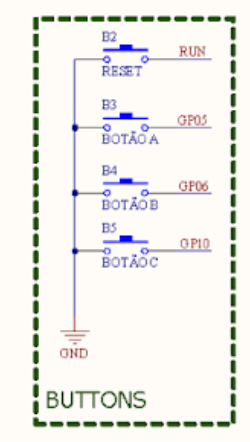
\includegraphics[width=0.6\textwidth]{circuito_botoes.png}
    \caption{Conexão dos botões ao RP2040.}
    \label{fig:circuito_botoes}
\end{figure}

\subsection{Debounce, Polling e IRQ}
\textbf{Funcionalidade:} Confirmar a alternância do LED nos dois modos.  

\textbf{Latência:} O aumento da carga no modo Polling provoca maior latência, enquanto o uso de IRQ garante resposta mais imediata.  

\textbf{Consumo de energia:} O IRQ é mais eficiente, pois evita que a CPU fique em espera constante.  

\textbf{Aplicações:} Polling pode ser suficiente em sistemas simples (ex.: leitura periódica de sensores), enquanto IRQ é essencial em sistemas críticos (ex.: teclados, comunicações seriais).  

\subsection{Tabela Comparativa -- Polling × IRQ}
A Tabela \ref{tab:polling_irq} resume a comparação entre Polling e IRQ.  

\begin{table}[H]
    \centering
    \begin{tabular}{lcc}
        \toprule
        Critério & Polling & IRQ \\
        \midrule
        Latência percebida & Maior & Menor \\
        Perdas de eventos  & Possível & Improvável \\
        Consumo de CPU     & Elevado & Reduzido \\
        Complexidade       & Baixa  & Maior \\
        Situações suficientes & Sistemas simples & --- \\
        Situações obrigatórias & --- & Sistemas críticos \\
        \bottomrule
    \end{tabular}
    \caption{Comparativo entre Polling e IRQ.}
    \label{tab:polling_irq}
\end{table}

% ---------------- Experiência 3 ----------------
\section{Experiência 3}

\subsection{Demonstração}
\textbf{Vídeo:} Disponível no YouTube em: \url{https://youtube.com/xxxxxx} \#EA701.  

\subsection{Comparação de código}
Comparar a simplicidade entre implementações em Python OO e em C modular, destacando clareza e manutenção do código.  

\subsection{Reflexão: IRQ + OO}
Discutir casos em que a combinação de IRQ e paradigma OO é vantajosa em sistemas embarcados reais (ex.: sistemas de tempo real, IoT e automação).  

\subsection{Expansão para 10 botões}
Discutir a viabilidade de Polling versus IRQ em um sistema com 10 botões. O Polling aumenta consideravelmente o consumo e a latência, enquanto o IRQ se mostra mais adequado.  

% ---------------- Conclusão ----------------
\section{Conclusão}
Neste roteiro, foram explorados os conceitos de GPIOs, LEDs RGB, botões, limites de tensão lógica, técnicas de tratamento de eventos (Polling e IRQ) e comparações entre paradigmas de programação (imperativo e OO) em C e Python.  

Os experimentos demonstraram diferenças significativas de desempenho entre C e MicroPython, além da importância da escolha correta entre Polling e IRQ de acordo com a aplicação. Como recomendação, projetos futuros devem considerar o uso de IRQ em sistemas mais complexos ou com múltiplos eventos assíncronos, e a escolha de linguagem/paradigma deve levar em conta tanto desempenho quanto legibilidade e manutenção do código.  

\end{document}
